\documentclass[conference]{IEEEtran}
\IEEEoverridecommandlockouts
% The preceding line is only needed to identify funding in the first footnote. If that is unneeded, please comment it out.
\usepackage{cite}
\usepackage{amsmath,amssymb,amsfonts}
\usepackage{algorithmic}
\usepackage{graphicx}
\usepackage{textcomp}
\usepackage{xcolor}
\usepackage{caption}
\usepackage{subcaption}
\usepackage{subfiles}
\usepackage{siunitx}
\usepackage{gensymb}

\graphicspath{{\subfix{../images/}}}
\def\BibTeX{{\rm B\kern-.05em{\sc i\kern-.025em b}\kern-.08em
    T\kern-.1667em\lower.7ex\hbox{E}\kern-.125emX}}
\begin{document}

\title{Conference Paper Title*\\
{\footnotesize \textsuperscript{*}Note: Sub-titles are not captured in Xplore and
should not be used}
\thanks{Identify applicable funding agency here. If none, delete this.}
}

\author{\IEEEauthorblockN{1\textsuperscript{st} Given Name Surname}
  \IEEEauthorblockA{\textit{dept. name of organization (of Aff.)} \\
    \textit{name of organization (of Aff.)}\\
    City, Country \\
    email address or ORCID}
  \and
  \IEEEauthorblockN{2\textsuperscript{nd} Given Name Surname}
  \IEEEauthorblockA{\textit{dept. name of organization (of Aff.)} \\
    \textit{name of organization (of Aff.)}\\
    City, Country \\
    email address or ORCID}
  \and
  \IEEEauthorblockN{3\textsuperscript{rd} Given Name Surname}
  \IEEEauthorblockA{\textit{dept. name of organization (of Aff.)} \\
    \textit{name of organization (of Aff.)}\\
    City, Country \\
    email address or ORCID}
}

\maketitle

\begin{abstract}
  With the growth of robotics, mobile robots are increasingly becoming a common aspect in key sectors of the economy. When compared to wheeled and tracked robots, legged robots present greater mobility and maneuverability, but less locomotion stability, which in turn demands more complex control systems. This paper aims to develop a quadruped robot capable of walking when teleoperated and assess its locomotion performance based on experiments. The first part of the methodology was dedicated to research and the definition of the robot's concept. The following stage involved the development of the robot's software, simulation, and, in parallel, the design, fabrication and assembly of the prototype. After both stages were done, the software was integrated into the prototype. After the integration stage, the locomotion experiments were conducted. Based on these experiments, it was possible to conclude that the robot was able to perform gaits of different sizes and walk in both plane and uneven terrains. Furthermore, it was observed that the body's rotation PID controller contributed to reducing the oscillation of the robot's body in both roll and pitch during walking in both terrains.
\end{abstract}

\begin{IEEEkeywords}
  Quadruped robot; Locomotion; Control.
\end{IEEEkeywords}

\section{Introduction}
Com o avanço da robótica, robôs móveis estão cada vez mais ganhando espaço em setores chave da economia como o comercial, industrial e militar. Os robôs terrestres que se locomovem com pernas têm se mostrado mais eficientes para se locomover em terrenos unevenes, inclinados e escorregadios, e também para superar obstáculos \cite{X.134}. Quando comparados com robôs com rodas, robôs com pernas ainda possuem melhor mobilidade e manobrabilidade em ambientes complexos, o que possibilita transitar por caminhos não necessariamente contínuos. Entre os robôs com pernas, os quadrúpedes vêm ganhando destaque por apresentarem maior estabilidade e uma estrutura mais simples quando comparados aos bípedes e hexápodes \cite{Shi2021}.

O uso de uma plataforma com quatro pernas requer um sistema de locomoção robusto que envolve o controle de equilíbrio da plataforma, o controle das juntas do robô e o planejamento de marchas. Para poder aplicar todos esses conceitos e desenvolver aplicações reais com robôs quadrúpedes, é fundamental estudar sua estrutura física, os tipos de marcha que eles podem realizar e os métodos de controle de locomoção que são utilizados nesses robôs.

O objetivo deste trabalho é desenvolver um sistema robótico do tipo quadrúpede capaz de se locomover de forma estável quando teleoperado. Serão estudados aspectos construtivos, de locomoção e de controle desse tipo robô. Além disso, será projetado um protótipo que será simulado e fabricado, a fim de testar os algoritmos de locomoção não apenas em um ambiente virtual, mas também na prática. Por fim, serão realizados experimentos de performance de locomoção com o protótipo físico, os quais analisarão a estabilidade do robô em ambientes de terreno plano e uneven.

A seção \ref{sec:the_quadruped_robot} tratará dos conceitos estudados para o desenvolvimento do robô. A seção \ref{sec:methodology} explicará a metodologia utilizada durante o projeto. Na seção \ref{sec:the_caramel}, será apresentado o Caramelo, o robô desenvolvido para essa pesquisa. A seção \ref{sec:results} apresentará os resultados dos testes e experimentos realizados, ao passo que a seção \ref{sec:conclusion}, as conclusões feitas a partir dos resultados. Por fim, a seção \ref{sec:final_points} apresentará as considerações finais e as sugestões dos autores para trabalhos futuros.

\section{Robot Development}

A small quadruped was designed and developed for research (Fig. X).
During the prototyping phase, the hardware architecture and physics structure was designed. Following that, the structure of the robot was printed and integrated with the hardware components. The robot's actuators are servo motors of the model dynamixel MX-28, and a Raspberry Pi 4 was chosen as processing unit. Furthermore, it contains an inertial sensor, model MPU6050. All the software was developed with the Robot Operating System 2 Humble (ROS 2) \cite{ROS2Humble}.

IMAGEM DO ROBO

The robot's structure is mammal-type, which is characterized by the presence of two joints in the sagittal plane, similar to animals such as dogs and horses.  The robot’s legs follow a configuration called full-elbow, in which the four legs are oriented backward, as shown in Fig. X. Furthermore, it features 3 degrees of freedom (DoF) per leg, providing the legs with substantial freedom of movement. The robot was designed to favor the mass balance between the body and the robot's legs, that is, the majority of its mass is in located in the body or as close to it as possible. Lighter legs can move quickly without significantly changing the center of gravity of the robot, which increases the stability and requires less control complexity.  On the other hand, the legs should be strong enough to support the robot's weight and the impact with the ground. 

The internal components, which include sensors, processing unit, and the communication interface with the actuators were arranged symmetrically in the robot's body. The actuators (components that contribute with most of the system's mass) were positioned as close as possible to the body. The motor that acts on the tibia joint was placed in the upper part of the femur, in order to reduce the moment of inertia of the leg. This choice required the addition of a transmission system between the engine and the tibia link, consisting of a rigid metal rod with a ball joint at each edge.

Quadruped robots move according to a gait pattern. The gait implemented for the robot follows the sequence of phases demonstrated in Fig. \ref{fig:trot_pattern}, in which the white rectangles represent the  swing phase and the gray rectangles represent the stance phase. During the stance phase, the legs are on the ground and push the robot in the desired direction.  In the swing phase, the legs are raised and moved to the next support point. This gait pattern is called a trot, and is based on the concept of periodic and symmetrical gaits. The periodic gaits are characterized by the continuous repetition of the movements in the same instants. The symmetry is a characteristic of gaits that move a pair of legs together, leaving and returning to the ground in a synchronized way. Although the structure of the robot makes it possible to perform other types of gaits, in this work, only the trot was considered. In order to reduce the control complexity, a discontinuous gait was adopted, that is, the robot's body moves only when all the legs are on the ground, resulting in an intermittent movement. In Fig. \ref{fig:trot_pattern}, it is noticeable that the same pair of diagonal legs always move at the same instant. Between two consecutive swing phases, there is a moment when all legs are in stance, which is when the robot body is displaced in the desired direction of locomotion.

\begin{figure}[!htb]
  \centering
  \caption{Padrão de movimentação da marcha para cada perna.}
  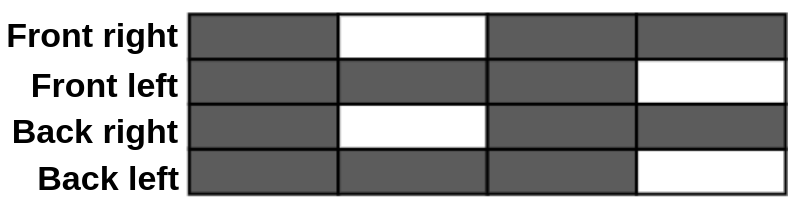
\includegraphics[width=0.45\textwidth]{trot_pattern.png}
  \vfill
  Fonte: autores.
  % \vspace{-\baselineskip}
  \label{fig:trot_pattern}
\end{figure}

The control subsystem of the robot is composed of two main components: the body's stabilization controller and 
joints' controllers. The body's stabilization controller is responsible for controlling the pitch and roll angles of the robot, maintaining it at 0 degrees. Meanwhile, the joints' controllers, each one a PID, are responsible for controlling each joint of the robot independently. 

The gait planner is responsible for controlling each leg and the robot's body. It defines where each foot will step and where the body should move to based on the desired velocity command. The gait planner uses a trajectory planner to calculate the trajectory each foot and body should follow. This trajectory is calculated based on the velocity command. The points of this trajectory are converted into the angles of the joints through the kinematic model. The kinematic model of the robot is responsible for mapping the three-dimensional position of the foot to the joints' angles of the respective leg.

The gait planner sends the points at which each foot must be at a frequency of $\SI{50}{\hertz}$. This frequency was defined as being the highest that the robot processing system was able to support and by respecting the Nyquist theorem, which indicates that in this case, the frequency should be greater than $\SI{4}{\hertz}$ --- since the step period is $0.5 s$.

% TODO ref nyquist

\subsection{Modelo cinemático do Caramelo}
\label{sec:detail_inv_kinematics}

Como dito anteriormente, o modelo cinemático é utilizado para resolver a cinemática inversa e a cinemática direta do robô. Para a cinemática direta, foi utilizado o pacote \textit{tf2}, um recurso disponível no \textit{ROS2} que facilita o gerenciamento de transformações entre eixos de coordenadas. A cinemática inversa, por outro lado, foi feita com base em uma análise geométrica. As variáveis $\theta_1$, $\theta_2$ e $\theta_3$ expressam a posição angular de cada uma das juntas de uma perna do robô e são calculadas com auxílio das equações \ref{eq:theta1} a \ref{eq:B} em função da posição $(x_{IK}, y_{IK}, z_{IK})$ desejada para a pata e dos comprimentos $L_1$, $L_2$ e $L_3$ (figura \ref{fig:caramel_tfs}).
\begin{equation}
  \label{eq:theta1}
  \theta_1 = \arctan{(\frac{x_{IK}}{y_{IK}})} - \arctan{(\frac{L_1}{a})}
\end{equation}
\begin{equation}
  \label{eq:theta2}
  \theta_2 = \frac{\pi}{2} - \arctan{(\frac{a}{z_{IK}}}) - \arctan{(\frac{\sqrt{1-A^2}}{A})}
\end{equation}
\begin{equation}
  \label{eq:theta3}
  \theta_3 = \arctan(\frac{\sqrt{1-B^2}}{B})
\end{equation}
\begin{equation}
  \label{eq:a}
  a = \sqrt{x_{IK}^2+y_{IK}^2-L_1^2}
\end{equation}
\begin{equation}
  \label{eq:A}
  A =\frac{a^2+z^2+L_2^2-L_3^2}{2L_2\sqrt{a^2+z_{IK}^2}}
\end{equation}
\begin{equation}
  \label{eq:B}
  B = \frac{a^2+z_{IK}^2-L_2^2-L_3^2}{2L_2L_3}
\end{equation}

\begin{figure}[htbp]
  \centering
  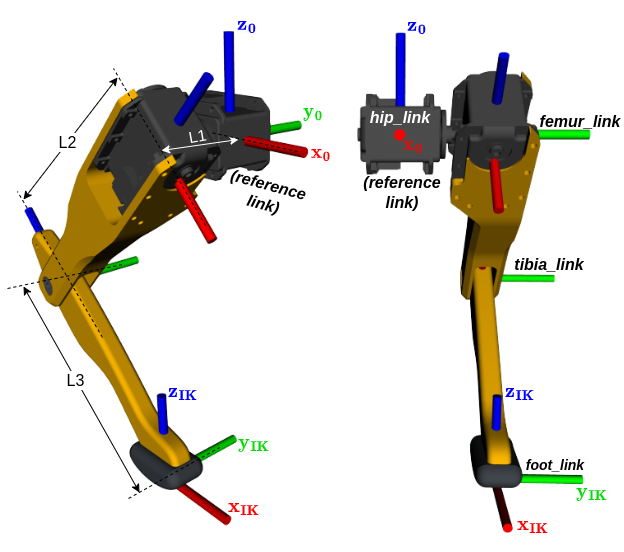
\includegraphics[width=0.4\textwidth]{caramel_tfs.png}

  \caption{Links da perna do robô.}
  Fonte: autores.
  \label{fig:caramel_tfs}
\end{figure}

Essas equações são úteis para o cálculo da posição de uma única perna, mas são insuficientes para realizar a cinemática do corpo do robô. Desta forma, um \textit{frame} central, chamado de \textit{base\_link} (figura \ref{fig:caramel_body}), é utilizado como referência, e uma matriz $T_M$ (eqs. \ref{eq:Tm} e \ref{eq:Rxyz}) é utilizada para realizar a cinemática do corpo, a partir das translações $(x_c, y_c, z_c)$ e rotações $(\alpha, \beta, \gamma)$ desejadas, sendo possível controlar cada um dos 6 graus de liberdade. Para tanto, as transformações $T_{FR}$, $T_{FL}$, $T_{BL}$ e $T_{BR}$ de cada um dos ombros (\textit{hip\_links}) em relação ao \textit{base\_link} são necessárias.
\begin{equation}
  \label{eq:Tm}
  T_M =
  \begin{bmatrix}
      &         &   & x_c \\
      & R_{xyz} &   & y_c \\
      &         &   & z_c \\
    0 & 0       & 0 & 1
  \end{bmatrix}
\end{equation}
\begin{equation}
  \label{eq:Rxyz}
  \begin{split}
    R_{xyz} =
    \begin{bmatrix}
      1 & 0          & 0           \\
      0 & \cos\alpha & -\sin\alpha \\
      0 & \sin\alpha & \cos\alpha
    \end{bmatrix}
    \\.
    \begin{bmatrix}
      \cos\beta  & 0 & \sin\beta \\
      0          & 1 & 0         \\
      -\sin\beta & 0 & \cos\beta
    \end{bmatrix}
    \\.
    \begin{bmatrix}
      \cos\gamma & -\sin\gamma & 0 \\
      \sin\gamma & \cos\gamma  & 0 \\
      0          & 0           & 1
    \end{bmatrix}
  \end{split}
\end{equation}

\begin{figure}[htbp]
  \centering
  \vspace{-0.75cm}
  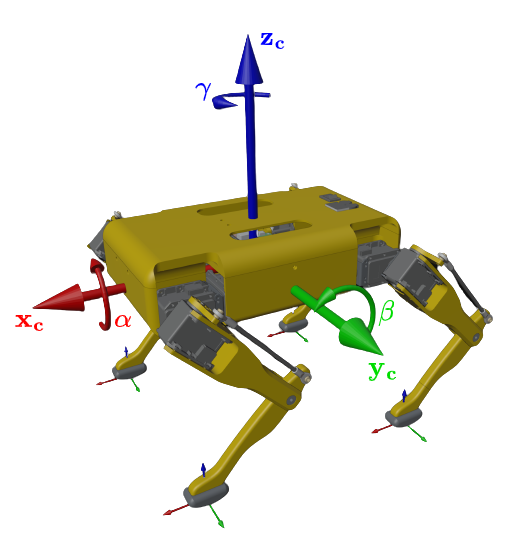
\includegraphics[width=0.35\textwidth]{caramel_body.drawio.png}

  \caption{Eixos do robô em posição de repouso.}
  Fonte: autores.
  \label{fig:caramel_body}
\end{figure}

O cálculo das angulações de cada perna então é feito utilizando como entrada os valores $(x_{IK}, y_{IK}, z_{IK})$ resultantes de cada uma das transformações, conforme a equação \ref{eq:xyzik}. O mesmo cálculo é feito para as demais pernas, utilizando  $T_{FL}$, $T_{BL}$ e $T_{BR}$.
\begin{equation}
  \label{eq:xyzik}
  \begin{bmatrix}
    x_{IK} \\
    y_{IK} \\
    z_{IK} \\
    1
  \end{bmatrix}= (T_M.T_{FR})^{-1}.
  \begin{bmatrix}
    x \\
    y \\
    z \\
    1
  \end{bmatrix}
\end{equation}

Desta forma, a cinemática inversa é capaz de computar as angulações  $\theta_1$, $\theta_2$ e $\theta_3$ de cada uma das pernas a partir da posição $(x, y, z)$ das patas em relação ao link central do robô e às translações $(x_c, y_c, z_c)$ e rotações $(\alpha, \beta, \gamma)$ desejadas para o corpo. Entretanto, em muitos casos, é mais conveniente realizar o cálculo dos ângulos passando como entrada as posições $(x, y, z)$ das patas em relação à sua posição \textit{default}, ou seja, a posição do seu \textit{foot\_link} quando o robô está em seu estado de repouso (figura \ref{fig:caramel_body}). Para isso, é possível realizar, previamente ao cálculo das angulações, mais uma transformação, desta vez do \textit{base\_link} para cada uma das posições \textit{default} das patas (equação \ref{eq:xyzik_foot}).
\begin{equation}
  \label{eq:xyzik_foot}
  \begin{bmatrix}
    x_{ik} \\
    y_{ik} \\
    z_{ik} \\
    1
  \end{bmatrix}= (T_M.T_{FR})^{-1}.
  (F_{FR}.
  \begin{bmatrix}
    x \\
    y \\
    z \\
    1
  \end{bmatrix})
\end{equation}

\subsection{Controle de angulação}

Os controladores de angulação são dois controladores PID em paralelo, responsáveis por controlar a rotação de \textit{roll} e \textit{pitch} do corpo do robô. Eles atuam de forma independente, controlando a rotação do corpo em ambos os eixos simultaneamente. Ambos os controladores são iguais e foram implementados seguindo o modelo apresentado no diagrama de blocos da figura \ref{fig:pid}.

\begin{figure}[htbp]
  \centering
  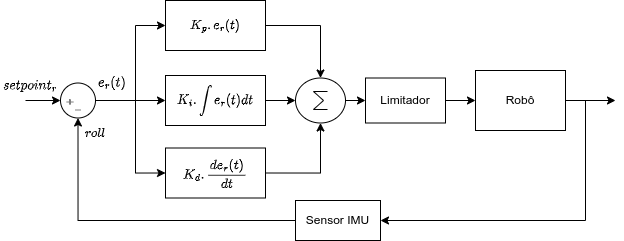
\includegraphics[width=0.48\textwidth]{PID.drawio.png}
  \caption{Controlador PID projetado.}
  Fonte: autores.
  \label{fig:pid}
\end{figure}

O IMU é o sensor responsável por medir a rotação do corpo do robô, possibilitando a realimentação das saídas do sistema. O limitador foi adicionado para evitar que sejam enviados valores que extrapolam os limites de rotação das juntas do robô. Os esforços de controle são enviados para o planejador de marchas que, por sua vez, envia os comandos de movimentação para os controladores das juntas.

\subsection{Trajectory planner}

The trajectory planner is responsible for calculating the trajectory that each foot must perform. For both stance and swing phases, a cycloidal curve is adopted. As shown in \cite{Shi2021}, a cycloidal curve can be defined in the three-dimensional space by (\ref{eq:traj_x}) to (\ref{eq:traj_k})
between the points $(x_o, y_o, z_o)$ and $(x_f, y_f, z_f)$ as a function of time $t$, step height $H$, and period $T$.
\begin{equation}
  x = (x_f - x_o) \frac{K - \sin{(K)}}{2 \pi} + x_o
  \label{eq:traj_x}
\end{equation}
\begin{equation}
  y = (y_f - y_o) \frac{K - \sin{(K)}}{2 \pi} + y_o
  \label{eq:traj_y}
\end{equation}
\begin{equation}
  z = H \frac{1 - \cos{(K)}}{2} + z_o
  \label{eq:traj_z}
\end{equation}
\begin{equation}
  K = \frac{2 \pi t}{T}
  \label{eq:traj_k}
\end{equation}

The graph of a cycloidal curve in 3D space is shown in Fig. \ref{fig:traj_space}. The same trajectory is illustrated in Fig. \ref{fig:traj_time} as a function of time. It is noticeable that the curve has the first null derivative when the foot touches the ground, which is favorable to open loop control, since the smoother the landing, the fewer disturbances are caused in the system.

\begin{figure*}[h]
  \centering
  \begin{subfigure}[t]{0.32\textwidth}
    \centering
    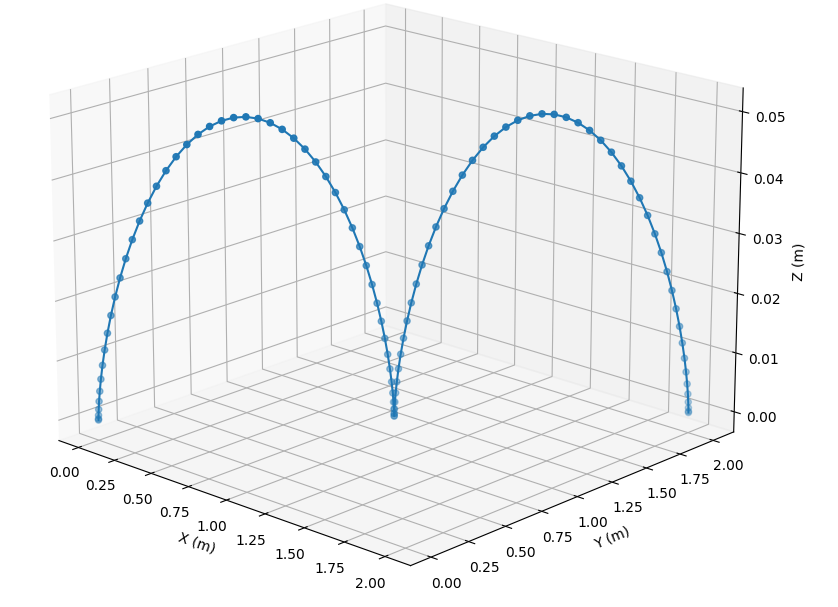
\includegraphics[width=1.0\textwidth]{Cycloid_space.png}
    \caption{Curva no espaço 3D.}
    \label{fig:traj_space}
  \end{subfigure}
  \begin{subfigure}[t]{0.32\textwidth}
    \centering
    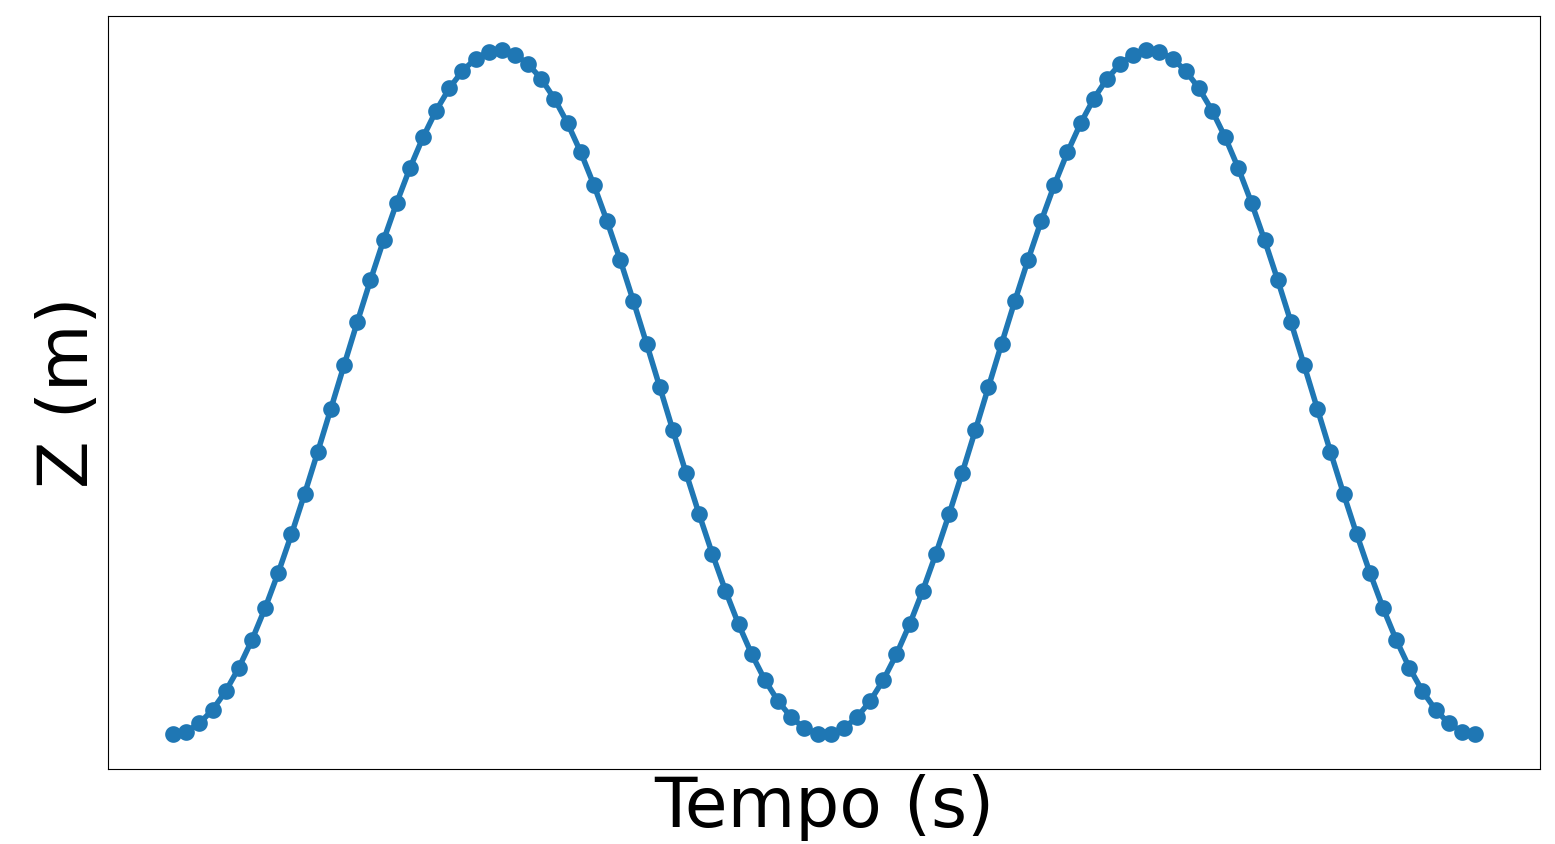
\includegraphics[width=1.0\textwidth]{Cycloid_time.png}
    \caption{Curva no tempo.}
    \label{fig:traj_time}
  \end{subfigure}
  \begin{subfigure}[t]{0.32\textwidth}
    \centering
    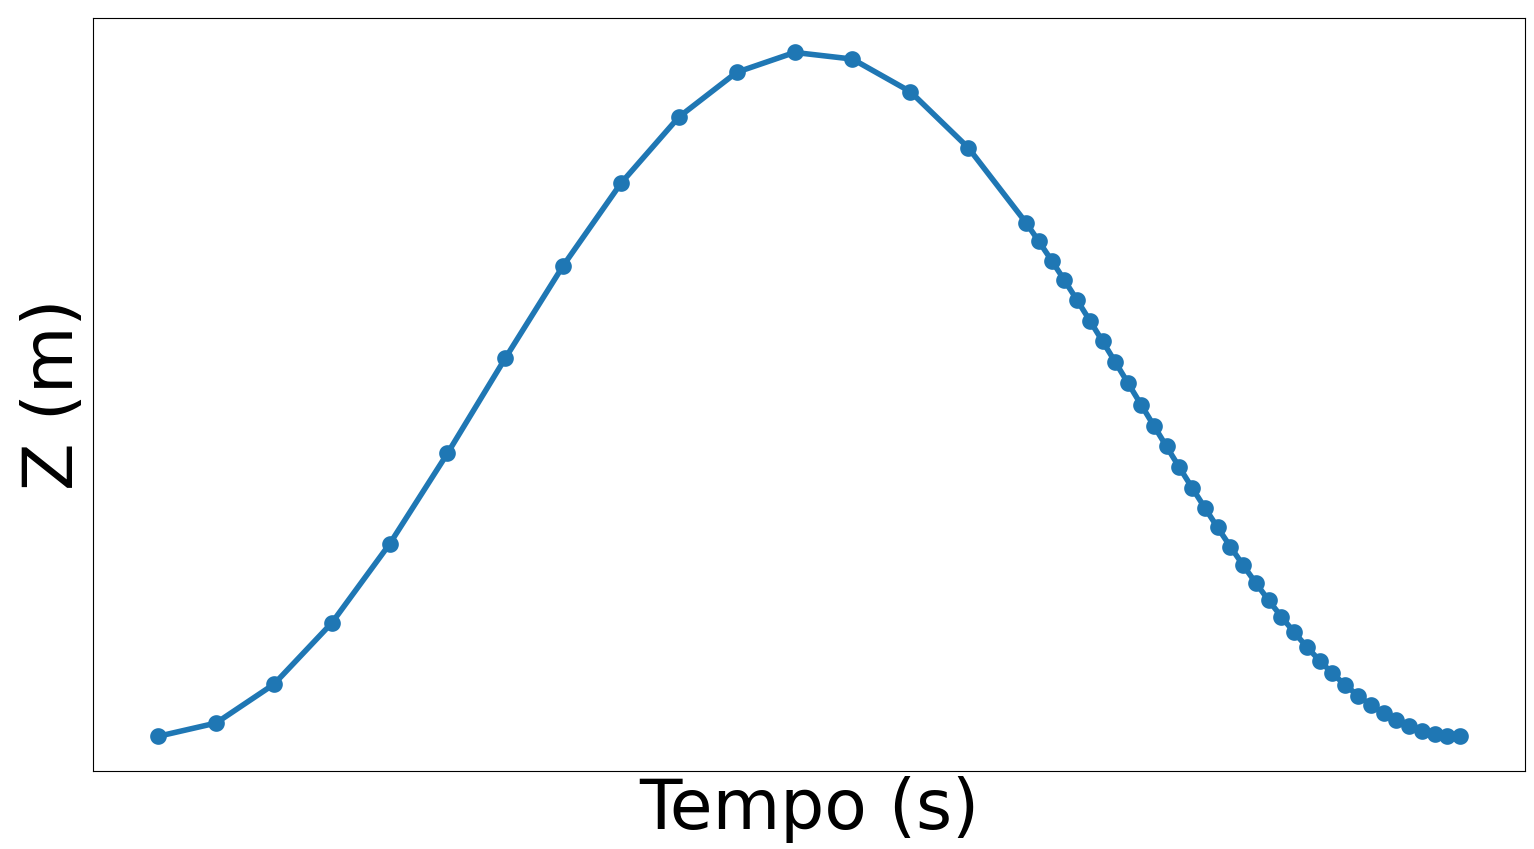
\includegraphics[width=1.0\textwidth]{Cycloid_modified.png}
    \caption{Curva com disposição de pontos modificada.}
    \label{fig:traj_time_modified}
  \end{subfigure}
  \vfill
  \caption{Trajetórias cicloidais para o passo de robô.}
  Fonte: autores.
  \label{fig:traj_curve}
\end{figure*}

In addition to the step height, the $x$ and $y$ translations, and the period, the robot's trajectory planner also considers two parameters to make the landing of the foot smoother. Since the robot’s actuators are servo motors controlled by position, the torque is proportional to the displacement it must perform between the points of the trajectory. Therefore, the higher the resolution of the trajectory, the smoother the movement. However, the resolution of the trajectory $N$ is fixed, given as a function of the step period and the frequency of the gait planner ($\SI{50}{\hertz}$) $N = 50T$. Thus, the strategy adopted is to distribute the $N$ points unevenly throughout the step period, so that there are more points near the moment the foot lands on the ground and less points near the moment the foot takes off. The $P_T$ parameter is a fraction of the total step period, and the $P_N$ is the fraction of the total number of points that should be between $0$ and $P_T \cdot T$. In other words, if $P_T = 0.66$ and $P_N = 0.33$, $33\%$ of $N$ will be in the first two-thirds of the period, while the remaining $67\%$ will be in the final one-third. The trajectory, considering these parameters, is illustrated in Fig. \ref{fig:traj_time_modified}.

\section{Results}

To assess the robot's locomotion performance with the implemented stabilization controller, the robot's capability of following a forward velocity setpoint and the oscillation of its body while walking were evaluated. An experiment was conducted, in which the robot should walk in a straight line of 1.5 meters in both flat and uneven terrain, with and without the stabilization controller, totalizing four tests. The flat terrain consisted of a cement floor and the uneven terrain, a ground formed by small loose stones. Both are illustrated in Fig. \ref{fig:terreno_plano} and \ref{fig:terreno_uneven}, respectively.

\begin{figure}[htbp]
  \centering
  \begin{subfigure}[htbp]{0.24\textwidth}
    \centering
    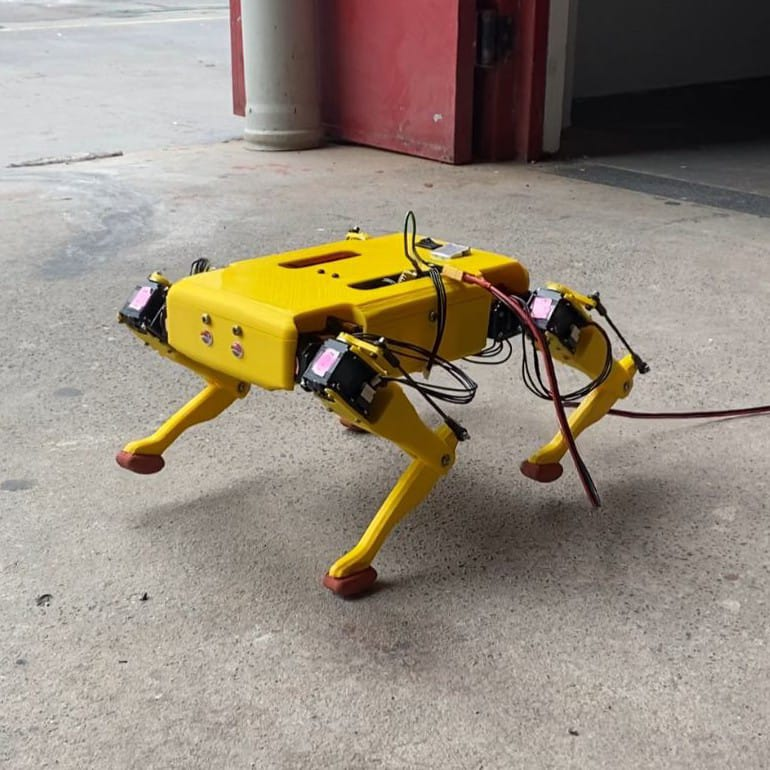
\includegraphics[width=1.0\textwidth]{terreno_plano.jpeg}
    \caption{Flat.}
    \label{fig:terreno_plano}
  \end{subfigure}
  \begin{subfigure}[htbp]{0.24\textwidth}
    \centering
    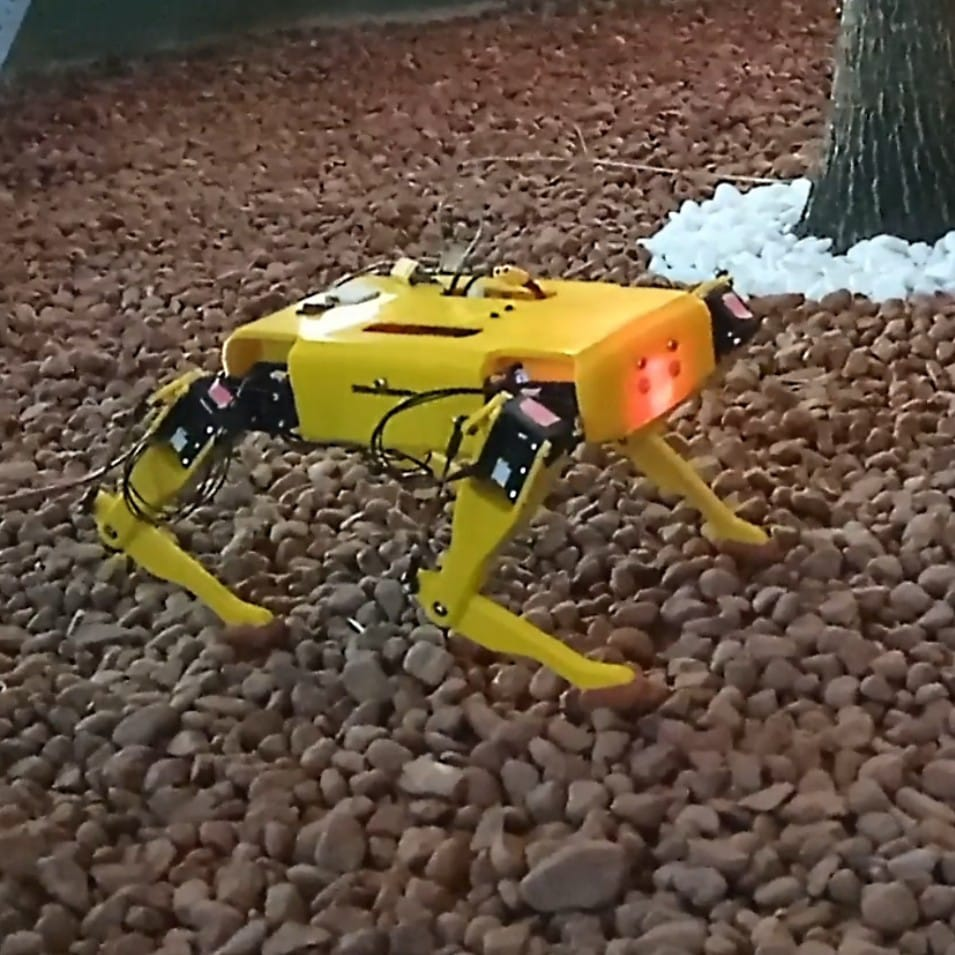
\includegraphics[width=1.0\textwidth]{terreno_irregular.jpeg}
    \caption{Uneven.}
    \label{fig:terreno_uneven}
  \end{subfigure}
  \vfill
  \caption{Terrains used for the experiment}
  \label{fig:terrenos}
\end{figure}

For each test, the robot received a forward velocity command of 0.05 m/s, and its mean velocity, as well as its pitch and roll oscillation, were recorded. The mean velocity was calculated based on the time it took to travel 1.5 meters and the oscillation is the difference between the maximum and minimum readings of the IMU. The calculated velocity was compared to the desired velocity sent to the robot and the stability data was analyzed statistically: first, the Shapiro-Wilk test \cite{leotti2005comparaccao} was applied to the distribution to check whether the distribution was normal; lastly, the results were compared by performing an Analysis of Variance (ANOVA) \cite{cano2012six}.

For all the tests, the robot's gait settings consisted of a height of 5 cm, a period of 0.5 seconds, a resolution of 25 points, $P_T$ = 0.66, and $P_N$ = 0.33. For each test type, 10 samples were collected.

%TODO incluir descrição da tabela
Table \ref{tab:vel_stab} summarizes the collected results. The robot did not reach a velocity of 0.05 m/s in any test. This result is due to errors in the final position of each leg during the swing phase: the legs could not reach the desired $(x,y)$ position required to maintain the desired velocity. The fact that the final position of one foot is a function of its motors' final orientation indicates that the motors did not reach their desired orientation. Before the experiment, the gait movement was tested with the legs off the ground (almost no load), and no significant errors were noted. Since the errors only appeared while walking, it is perhaps caused by the fact that the motors were not powerful enough to support the robot's weight appropriately while walking.

\begin{table}[!htb]
  \centering
  \caption{Velocity and stability results}
  \begin{tabular}{ccccc}
    \hline
    \textbf{Test}              & \textbf{1}   & \textbf{2}  & \textbf{3}   & \textbf{4}   \\ \hline
    Ter.                       & Flat         & Flat        & Uneven       & Uneven       \\ \hline
    \begin{tabular}[c]{@{}c@{}}S. C. \end{tabular} & No           & Yes         & No           & Yes          \\ \hline
    \begin{tabular}[c]{@{}c@{}}Vel. \\ $(cm/s)$ \end{tabular} & 2.15         & 3.68        & 2.03         & 2.39         \\ \hline
    \begin{tabular}[c]{@{}c@{}} $\sigma_{Vel}$  \\ $(cm/s)$ \end{tabular} & 0.040        & 0.075       & 0.016        & 0.047        \\ \hline
    \begin{tabular}[c]{@{}c@{}} $\Delta_{Roll}$ \end{tabular} & 12.59\degree & 8.81\degree & 13.37\degree & 11.13\degree \\\hline
    \begin{tabular}[c]{@{}c@{}} $\sigma_{Roll}$ \end{tabular} & 2.54\degree  & 2.36\degree & 0.78\degree  & 1.47\degree  \\ \hline
    \begin{tabular}[c]{@{}c@{}} $\Delta_{Pitch}$ \end{tabular} & 11.55\degree & 8.31\degree & 15.19\degree & 12.09\degree \\ \hline
    \begin{tabular}[c]{@{}c@{}} $\sigma_{Pitch}$ \end{tabular} & 1.89\degree  & 2.63\degree & 1.44\degree  & 1.66\degree  \\ \hline
  \end{tabular}
  \label{tab:vel_stab}
\end{table}

In addition to the velocity results, the pitch and roll oscillations were compared to determine whether or not the stabilization controller lowered the robot's body oscillation. The Shapiro-Wilk test was applied to the data from all the tests, after removing outliers, and every test returned a $\text{p-value} > 0.05$, which indicates that all the distributions followed a normal curve. The ANOVA was, then, applied to compare the roll and pitch oscillations from tests 1 and 2. The same process was applied to the tests 3 and 4 as well. The ANOVA revealed that the roll and pitch distributions of the tests with and without stabilization control were significantly different. Table \ref{tab:vel_stab} shows that the mean value of the tests with stabilization control was less than the mean value of the test without it, which proves that it indeed lowered the robot's body oscillations in both terrain types. Fig. \ref{fig:imu_test} better pictures the data distribution. Despite the more scattered distribution presented, 3 out of 4 of the tests with stabilization control had its third quartile less than the first quartile of the distribution without the controller for the same terrain type, demonstrating that the controller lowered the oscillations in $75\%$ of the collected test samples.

\begin{figure}[!htb]
  \centering
  \begin{subfigure}[t]{0.49\textwidth}
    \centering
    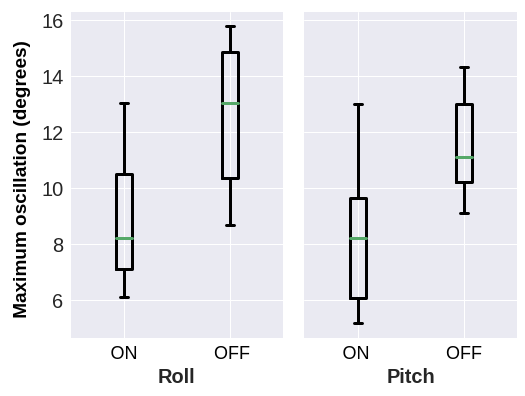
\includegraphics[width=1.0\textwidth]{plane_boxplot.png}
    \caption{Terreno plano.}
    \label{fig:imu_test_plane}
  \end{subfigure}
  \begin{subfigure}[t]{0.49\textwidth}
    \centering
    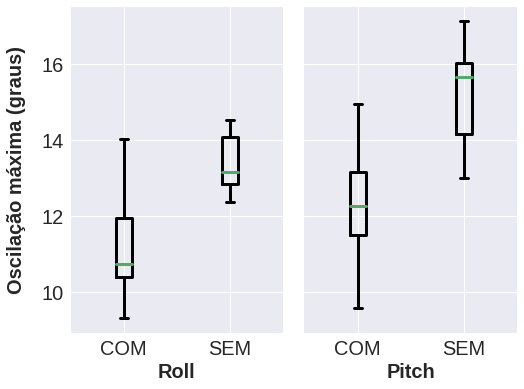
\includegraphics[width=1.0\textwidth]{irregular_boxplot.png}
    \caption{Terreno irregular.}
    \label{fig:imu_test_irregular}
  \end{subfigure}
  \caption{Oscilação do corpo em ambos os tipos de terreno.}
  Fonte: autores.
  \label{fig:imu_test}
\end{figure}

\section{Conclusion}

This paper addressed the design, prototyping and testing of a quadruped robot. An experiment was held to assess the robot's walking performance. The results showed that the robot did not reach the desired velocity in any of the tests. This was due to errors during the gait's swing phase, which indicates that the motors were unable to support the robot's weight while walking. These errors were not compensated, because the gait's trajectory tracking is open-loop (only the individual joint's controllers are closed-loop). In addition to that, it was possible to conclude that the implemented stabilization controller was able to lower the robot's body oscillations in pitch and roll while walking in both flat and uneven terrains.

Reviewing the robot's actuators is recommended for future work. Perhaps a model with more torque is required for more precise control performance.

The robot's project is open source and is available on GitHub \cite{CaramelRepo}.

\section*{Acknowledgment}

The preferred spelling of the word ``acknowledgment'' in America is without
an ``e'' after the ``g''. Avoid the stilted expression ``one of us (R. B.
G.) thanks $\ldots$''. Instead, try ``R. B. G. thanks$\ldots$''. Put sponsor
acknowledgments in the unnumbered footnote on the first page.

\section*{References}

Please number citations consecutively within brackets \cite{b1}. The
sentence punctuation follows the bracket \cite{b2}. Refer simply to the reference
number, as in \cite{b3}---do not use ``Ref. \cite{b3}'' or ``reference \cite{b3}'' except at
the beginning of a sentence: ``Reference \cite{b3} was the first $\ldots$''

Number footnotes separately in superscripts. Place the actual footnote at
the bottom of the column in which it was cited. Do not put footnotes in the
abstract or reference list. Use letters for table footnotes.

Unless there are six authors or more give all authors' names; do not use
``et al.''. Papers that have not been published, even if they have been
submitted for publication, should be cited as ``unpublished'' \cite{b4}. Papers
that have been accepted for publication should be cited as ``in press'' \cite{b5}.
Capitalize only the first word in a paper title, except for proper nouns and
element symbols.

For papers published in translation journals, please give the English
citation first, followed by the original foreign-language citation \cite{b6}.

\begin{thebibliography}{00}
  \bibitem{b1} G. Eason, B. Noble, and I. N. Sneddon, ``On certain integrals of Lipschitz-Hankel type involving products of Bessel functions,'' Phil. Trans. Roy. Soc. London, vol. A247, pp. 529--551, April 1955.
  \bibitem{b2} J. Clerk Maxwell, A Treatise on Electricity and Magnetism, 3rd ed., vol. 2. Oxford: Clarendon, 1892, pp.68--73.
  \bibitem{b3} I. S. Jacobs and C. P. Bean, ``Fine particles, thin films and exchange anisotropy,'' in Magnetism, vol. III, G. T. Rado and H. Suhl, Eds. New York: Academic, 1963, pp. 271--350.
  \bibitem{b4} K. Elissa, ``Title of paper if known,'' unpublished.
  \bibitem{b5} R. Nicole, ``Title of paper with only first word capitalized,'' J. Name Stand. Abbrev., in press.
  \bibitem{b6} Y. Yorozu, M. Hirano, K. Oka, and Y. Tagawa, ``Electron spectroscopy studies on magneto-optical media and plastic substrate interface,'' IEEE Transl. J. Magn. Japan, vol. 2, pp. 740--741, August 1987 [Digests 9th Annual Conf. Magnetics Japan, p. 301, 1982].
  \bibitem{b7} M. Young, The Technical Writer's Handbook. Mill Valley, CA: University Science, 1989.
\end{thebibliography}
\vspace{12pt}
\color{red}
IEEE conference templates contain guidance text for composing and formatting conference papers. Please ensure that all template text is removed from your conference paper prior to submission to the conference. Failure to remove the template text from your paper may result in your paper not being published.

\end{document}
